%!TEX root = ../../../main.tex

\subsection{Dimensionality Reduction Algorithms}

    Dimensionality reduction techniques are important in many applications related to machine learning.
    They aim to find low-dimensional embedding that should preserve sufficient information from the original dimension.
    Let's define $X = \{x_{ik}|i=(1,..,c);k=(1,..,n_{i})\}$ as training samples where $x_{ik} \in R^{d}$ is the $k^{th}$ sample of the $i^{th}$ class, $d^x$ is the original dimension of data, $d^y$ is the desired dimension of data after transformation such that $d^y < d^x$.

    \subsubsection{Linear discriminant analysis}
        The linear discriminant analysis (LDA) technique is developed to linearly transform the features into a lower dimensional space where the ratio of the between-class variance to the within-class variance is maximized, thereby guaranteering the optimal class separability.
        The projection results of $X$ on the lower dimensional space is denoted by $Y = \{y_{ik} = w^T x_{ik}|i=(1,..,c); k=(1,...,n_{i})\}$. $\boldsymbol{S}_B^y$ and $\boldsymbol{S}_W^y$ are computed as follows: 

        \begin{align}
            \boldsymbol{S}_W^y &= \sum_{i=1}^{c}\sum_{k=1}^{n_{i}}(y_{ik}-\mu_i)(y_{ik}-\mu_i)^T \label{eq:LDA_Sw_y}\\
            \boldsymbol{S}_B^y &= \sum_{i=1}^{c}n_i(\mu_i - \mu)(\mu_i - \mu)^T \label{eq:LDA_Sb_y}
        \end{align}

        where $\mu_i=\frac{1}{n_i}{\sum_{k=1}^{n_{i}}}{y_{ik}}$ is the mean of all samples of the $i^{th}$ class in the lower dimensional space; $\mu=\frac{1}{n}\sum_{i=1}^{c}{\sum_{k=1}^{n_{i}}{y_{ik}}}$ is the mean of all samples of all classes; $n=\sum_{i=1}^{c}n_i$ is the total number of data samples.
        The between-class $\boldsymbol{S}_B^y$ and within-class $\boldsymbol{S}_W^y$ covariance matrices in new dimension are not known yet but can be formulated as the linearly transformed versions of their counterparts $\boldsymbol{S}_B^x$ and $\boldsymbol{S}_W^x$ in original dimension.

        \begin{align}
            \boldsymbol{S}_W^y &= \omega^T\boldsymbol{S}_W^x\omega\\
            \boldsymbol{S}_B^y &= \omega^T\boldsymbol{S}_B^x\omega
        \end{align}

        $\boldsymbol{S}_B^x$ and $\boldsymbol{S}_W^x$ are simply calculable as follows:

        \begin{align}
            \boldsymbol{S}_W^x &= \sum_{i=1}^{c}\sum_{k=1}^{n_{i}}(x_{ik}-\mu_i^{(x)})(x_{ik}-\mu_i^{(x)})^T \label{eq:LDA_Sw_x}\\
            \boldsymbol{S}_B^x &= \sum_{i=1}^{c}n_i(\mu_i^{(x)} - \mu^{(x)})(\mu_i^{(x)} - \mu^{(x)})^T \label{eq:LDA_Sb_x}
        \end{align}

        Then the objective function is formulated by a Rayleigh quotient:

        \begin{equation}
            \boldsymbol{\omega}^* = \operatorname*{argmax}_{\boldsymbol{\omega}}\frac{trace(\boldsymbol{S}_B^y)}{trace(\boldsymbol{S}_W^y)} = \operatorname*{argmax}_{\boldsymbol{\omega}}\frac{trace(\omega^T\boldsymbol{S}_B^x\omega)}{trace(\omega^T\boldsymbol{S}_W^x\omega)}
            \label{eq:LDA}
        \end{equation}

        The Fisher's criterion in Equation \eqref{eq:LDA} can be reformulated as:

        \begin{equation}
            \boldsymbol{S}_W^x\omega = \lambda\boldsymbol{S}_B^x\omega
        \end{equation}

        where $\lambda$ represents the eigenvalues of the transformation matrix $\omega$. The analytical solution of $\boldsymbol{\omega}^*$ is a $(d^x \times d^y)$ matrix optained by calculating the eigenvectors $V = \{v_1,v_2,...,v_{d^x}\}$ sorted by the scalar values of corresponding eigenvalues $\lambda = \{\lambda_1,\lambda_2,...,\lambda_{d^x}\}$ of the matrix $\boldsymbol{S} = {\boldsymbol{S}_W^x}^{-1}\boldsymbol{S}_B^x$, then slice it till the largest $d^y$ element as illustrated in Figure \ref{fig:lda_solution}.

        \begin{figure}[htbp]
            \centering
            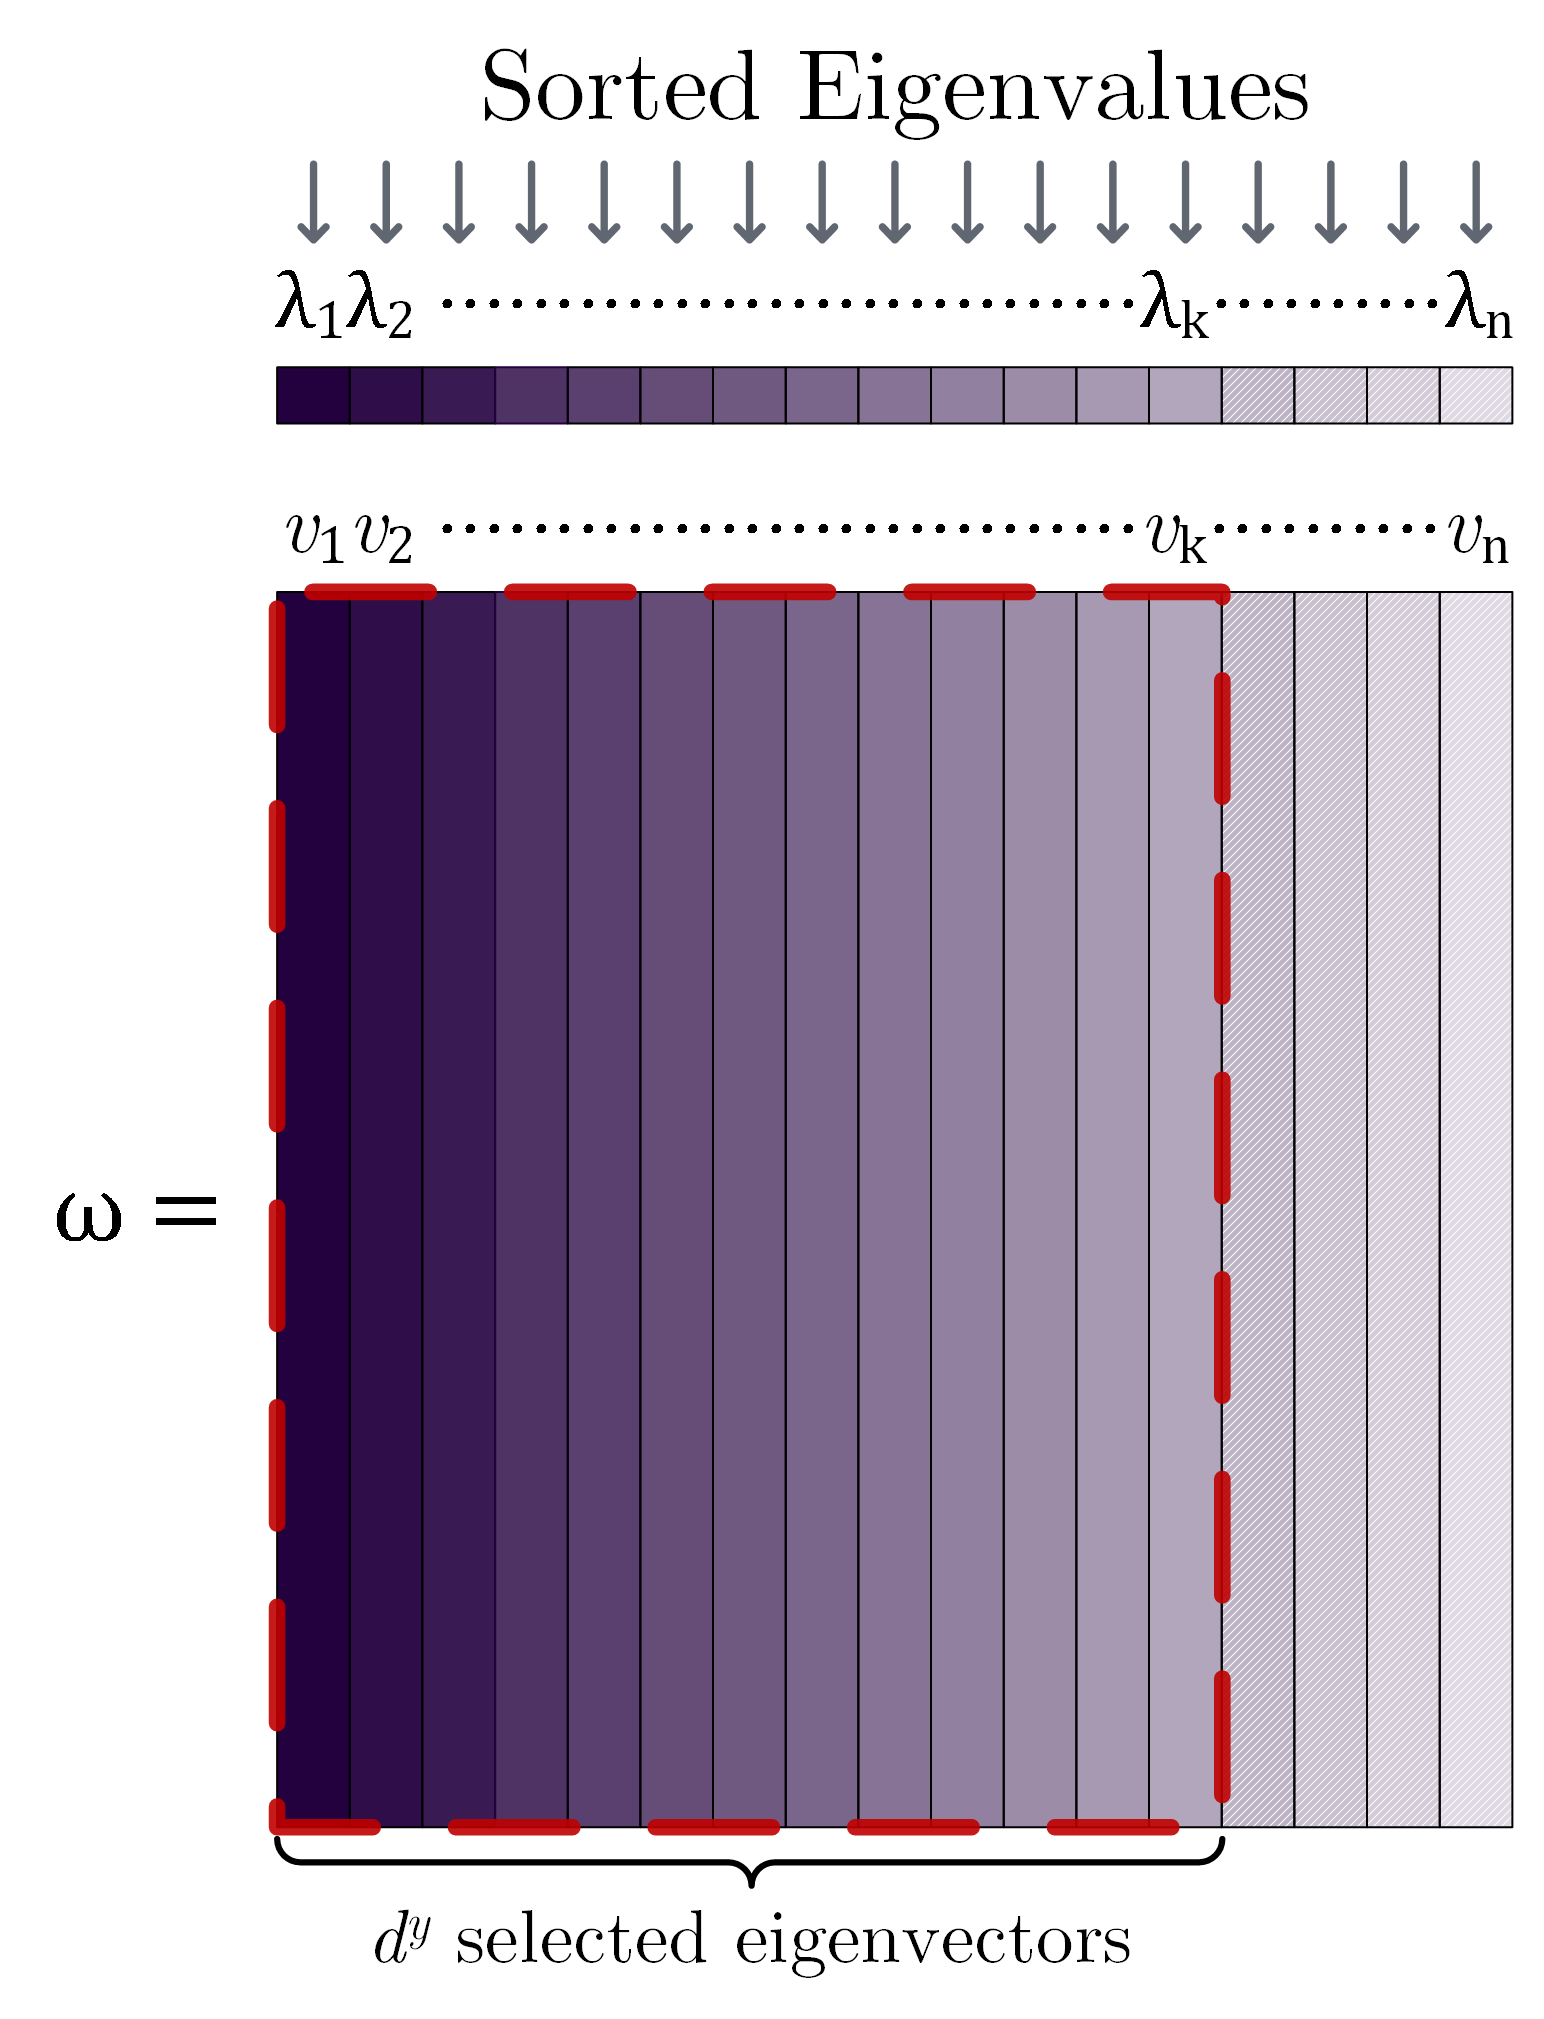
\includegraphics[width=0.4\linewidth]{figs/lda_solution.png}
            \caption{Analytical solution of LDA.}
            %\vspace{-0.3cm}
            \label{fig:lda_solution}
        \end{figure}

    \subsubsection{Pairwise-covariance linear discriminant analysis}
        Pairwise-covariance linear discriminant analysis (pc-LDA) is an extension of LDA introduced in \cite{kong2014pairwise} that overcomes it's drawbacks by formulating pairwise distances between pairs of classes.
        The pairs of $a$ and $b$ classes are regarded as two Gaussian distributions $\mathcal{N}_a(\mu_a,{\boldsymbol{S}_W^y}_a), \mathcal{N}_b(\mu_b,{\boldsymbol{S}_W^y}_b)$ and the objective distance between two classes is defined as their Kullback-Leibler divergence \cite{kullback1951}:

        \begin{equation}
            D_{KL}\left(\mathcal{N}_a\parallel\mathcal{N}_b\right)=\frac{1}{2}\left(\mu_a-\mu_b\right)^{T}{\left({\boldsymbol{S}_W^y}_{ab}\right)}^{-1}\left(\mu_a-\mu_b\right),
        \end{equation}

        where ${\boldsymbol{S}_W^y}_{ab}$ is pairwise covariance matrix (Equation \eqref{eq:pc-LDA_Sw_ab}), calculated as the $\beta$ parameterized convex sum of global within-class scatter matrix $\boldsymbol{S}_W^y$ used in LDA with the within-class scatter matrix of each class ${\boldsymbol{S}_W^y}_i$ (Equation \eqref{eq:pc-LDA_Sw_i}).
        The author theorizes it would better represent the data distribution within two classes.

        \begin{align}
            {\boldsymbol{S}_W^y}_i &= \sum_{j=1}^{v}\sum_{k=1}^{n_{ij}}{\left(y_{ik}-\mu_i\right)\left(y_{ik}-\mu_i\right)^T} \label{eq:pc-LDA_Sw_i}\\
            {\boldsymbol{S}_W^y}_{ab} &= \beta\frac{n_a{\boldsymbol{S}_W^y}_a+n_b{\boldsymbol{S}_W^y}_b}{n_a+n_b}+\left(1-\beta\right){\boldsymbol{S}_W^y}
            \label{eq:pc-LDA_Sw_ab}
        \end{align}

        where $n_a$ and $n_b$ are number of samples belonging to class $a$ and $b$. The final objective is properly weighted to focus on classes with more samples:

        \begin{equation}
            \operatorname*{min}_{\boldsymbol{\omega}}{J}=\sum_{a=1}^{c}\sum_{b=a+1}^{c}{\frac{n_an_b}{{[2D_{KL}\left(\mathcal{N}_a\parallel\mathcal{N}_b\right)]}^q}},\ \ s.t.\ \omega^T\omega=\boldsymbol{I}
            \label{eq:pc-LDA}
        \end{equation}

        here $q\ge1$ is a hyper-parameter that controls how much the pairs of classes with smaller objective distances are biased over the others.

        The new model of pc-LDA is solved with a variant of gradient descent described in \cite{kong2014pairwise}, where $\nabla J\left(\omega\right)$ is computed and $\omega$ is updated as Equation \eqref{eq:pc-LDA_omega} in order to enforce $\omega$ on the Stiefel manifold. Every several iterations, due to numerical error, the learnt transformation is unitarized $\omega \leftarrow \omega{\left(\omega^T\omega\right)}^{-\frac{1}{2}}$ to ensure that the constraint $\omega^T\omega = \boldsymbol{I}$ is satisfied.

        \begin{equation}
            \omega \leftarrow \omega - \eta\left(\nabla J - \omega{[\nabla J]}^T\omega\right)
            \label{eq:pc-LDA_omega}
        \end{equation}
